% !TEX root = main.tex

\section{Models}

\subsection{Logic Tensor Network (LTN)}

\begin{figure}
    \centering
    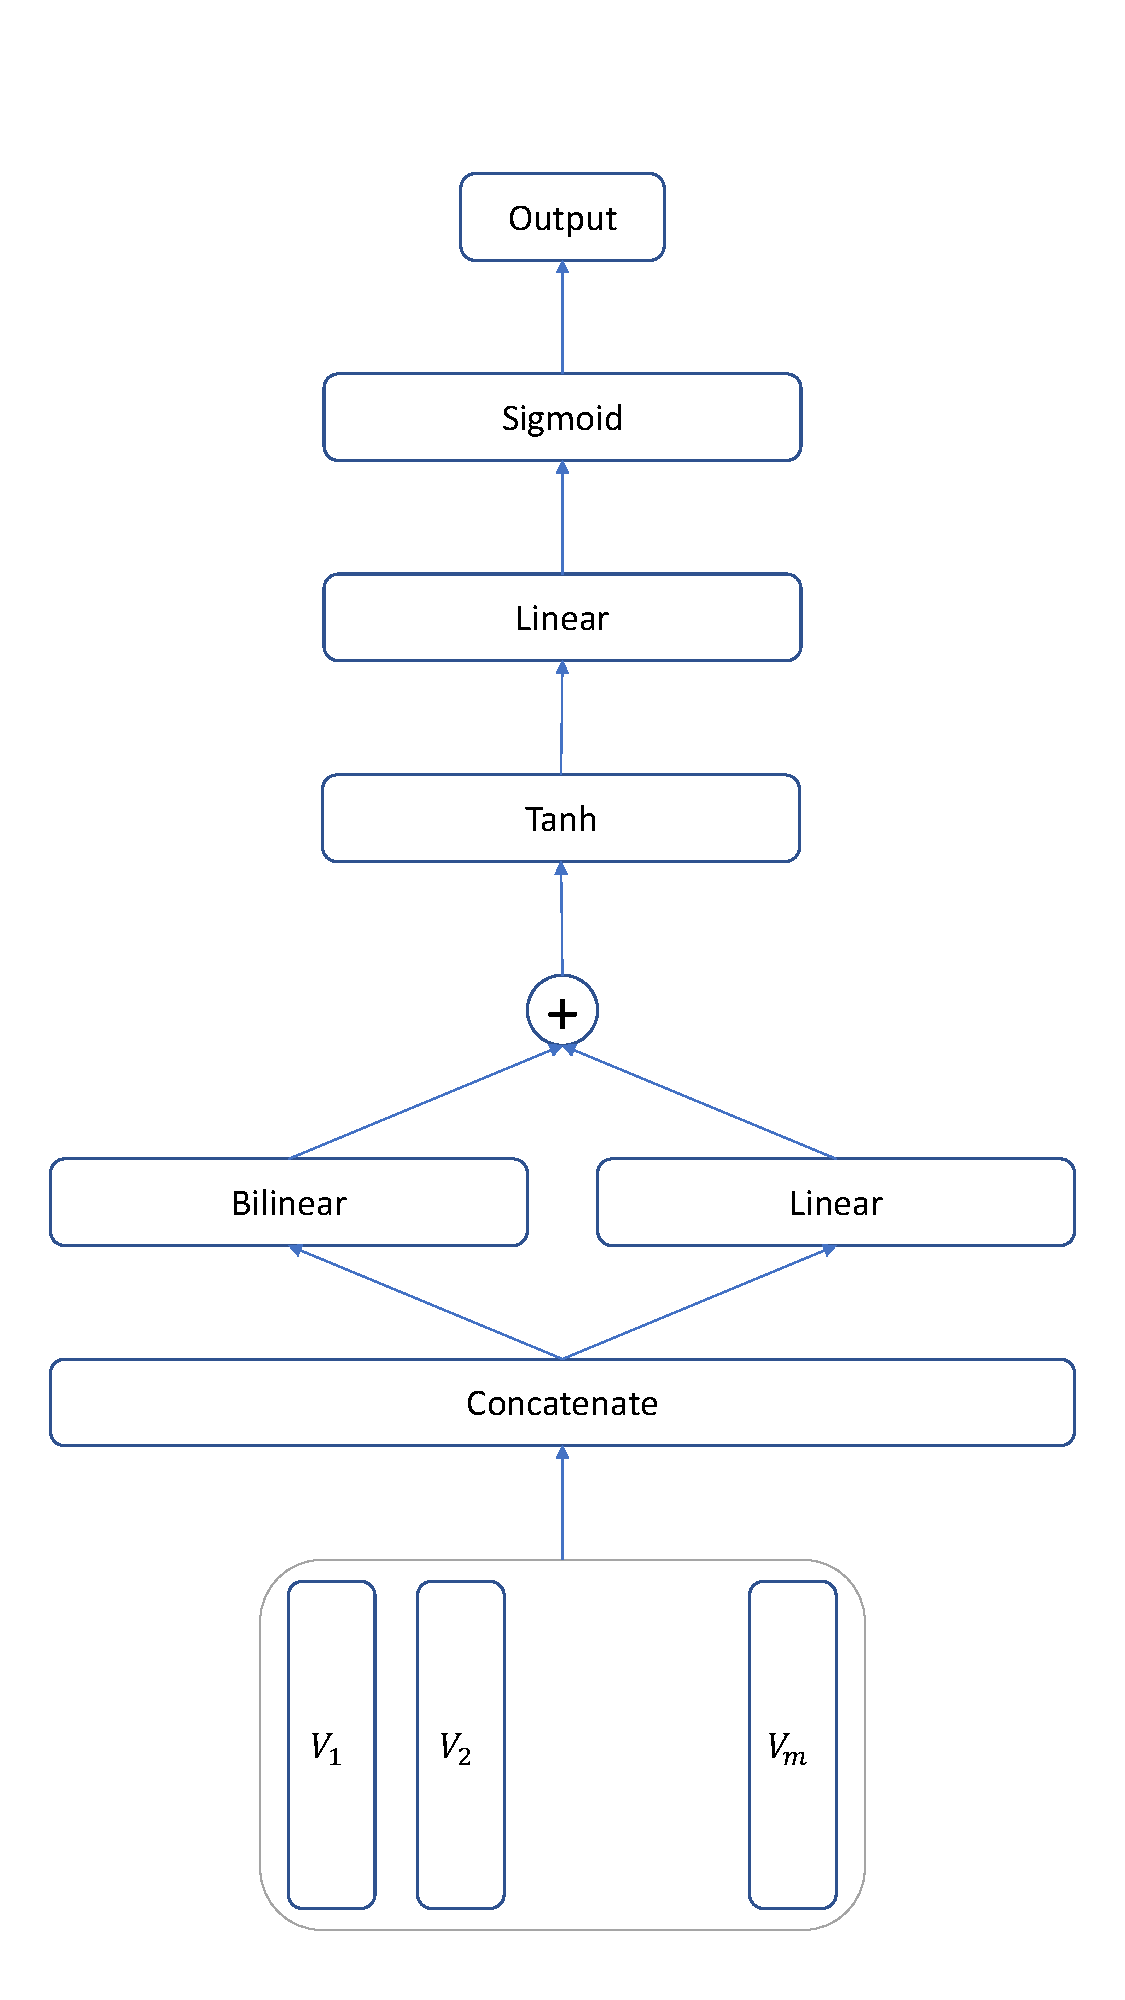
\includegraphics[width=.4\textwidth]{img/Predicate.pdf}
    \caption{Model for Predicate}
    \label{fig:LTN_predicate}
\end{figure}

\subsection{Convolutional Logic Tensor Network (CLTN)}

Here we first follow up the implementation of $G(c)$, $G(f)$, and $G(\phi)$. However, we tend to use Convolutional Neural Network to implement $G(p)$.

First we need to construct the input matrix with the $v_1,v_2,\dots,v_m$. From LTN model, we learned that the bilinear manipulation is critical to get a good performance. Here we use the idea of cross product. That is, take the cross product $x^Tx$ as

The model is illustrated in Figure \ref{fig:CLTN_predicate}.

\begin{figure}
    \centering
    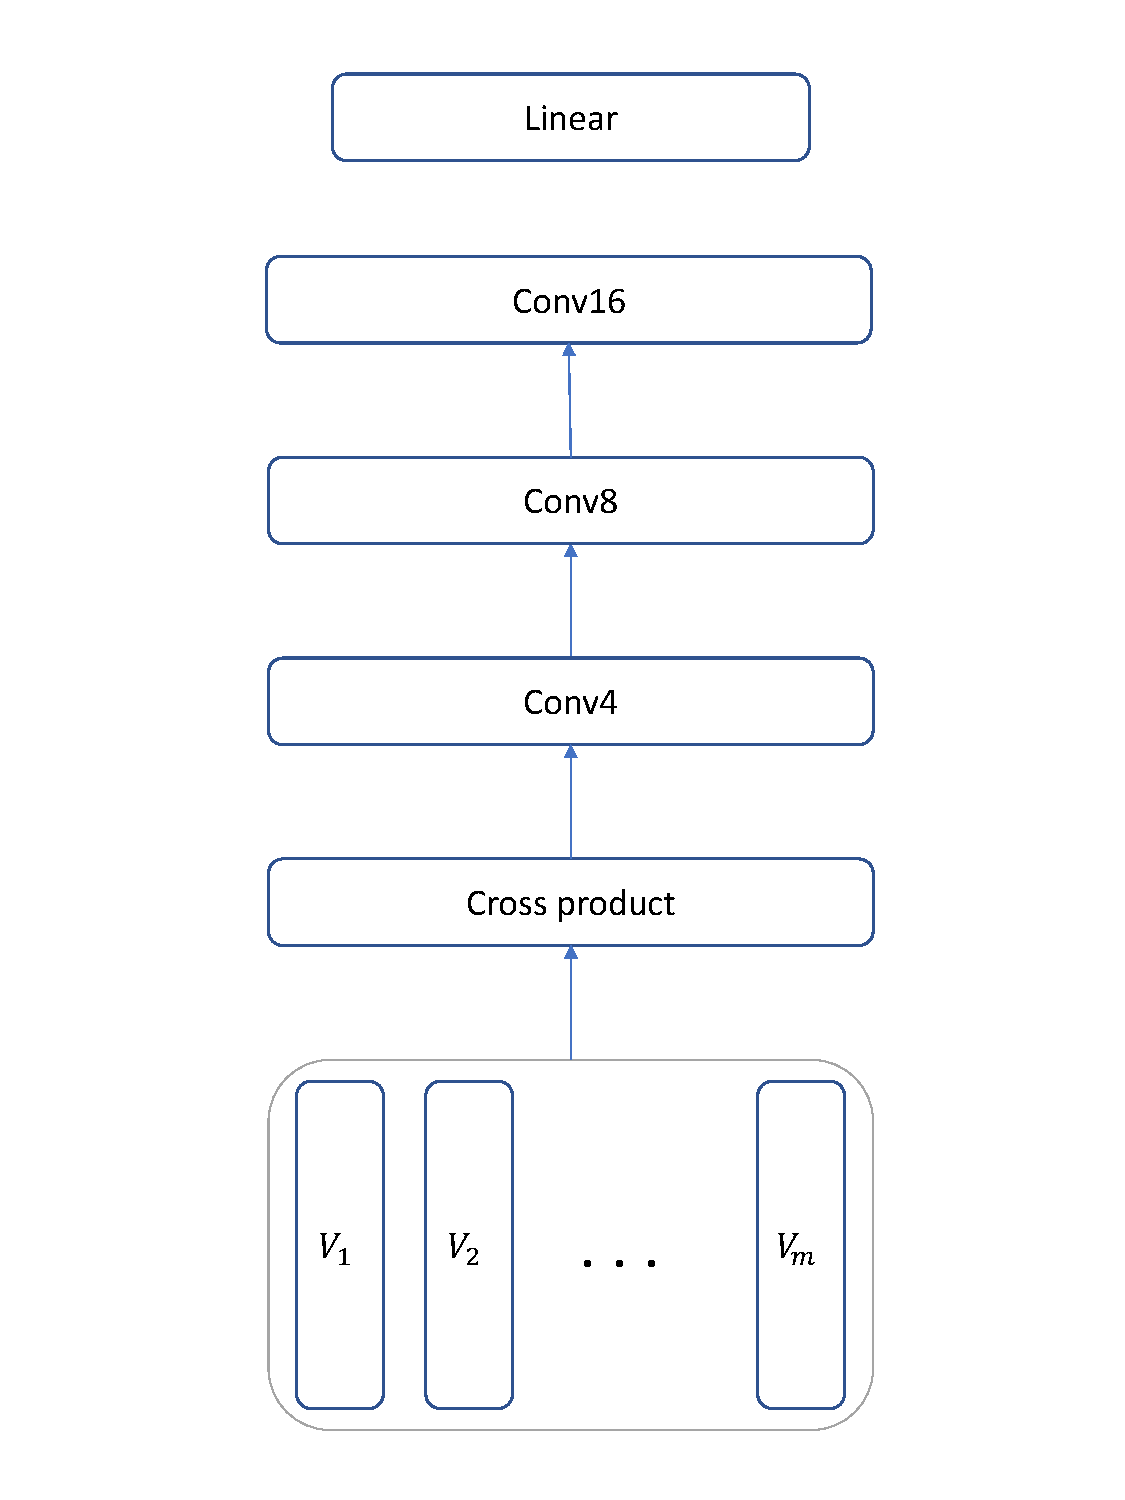
\includegraphics[width=.4\textwidth]{img/CLTN_Predicate.pdf}
    \caption{Model for Predicate}
    \label{fig:CLTN_predicate}
\end{figure}
